\documentclass{beamer}  
\usepackage{amsmath}
\usepackage{graphicx}
\usepackage{url}
\usepackage{fancyvrb}
\usepackage[pdftex]{color}

\mode<presentation>
{ \usetheme{Darmstadt} }

\title{Revisiting the Issue of Performance Enhancement of Discrete Event
Simulation Software
   \thanks{We wish to thank Victor Castillo and the Lawrence Livermore
   National Laboratory for supporting this research.}
}

\author{
Alex Bahouth, 
Steven Crites,
Norman Matloff and
Todd Williamson \\
Department of Computer Science \\
University of California at Davis \\
Davis, CA 95616 USA \\
matloff@cs.ucdavis.edu 
}

\date{}
 
\begin{document} 

\begin{frame}
\titlepage
\end{frame}

\begin{frame}
This presentation is produced using C. Campani's Beamer \LaTeX\ class.

See \url{http://heather.cs.ucdavis.edu/~matloff/beamer.html} for a quick
tutorial.

{\it Disclaimer:  Our slides here won't show off what Beamer can do.
Sorry. :-)}  

\end{frame}

\begin{frame}
\frametitle{Issues Addressed in This Paper}

\begin{itemize}

\item Interpreted languages (Java, Python) now popular for DES

\pause

\item Interpreted languages are slow.

\pause

\item DES literature mainly algorithm-centric.

\pause

\item What can be done specifically for interpreted languages?

\pause

\item What can be done for systems considerations, e.g. VM?

\end{itemize}

\end{frame}

\begin{frame}
\frametitle{Case Study:  SimPy}

Our investigation took the form of a case study:  enhancing the
peformance of the SimPy DES language.

\pause

About SimPy:

\begin{itemize}

\pause

\item Written by Klaus Muller and Tony Vignaux.

\pause

\item I have developed an online DES course based on SimPy, available
at \url{heather.cs.ucdavis.edu/~matloff/simcourse.html}.

\pause

\item SimPy uses Python:

\pause

   \begin{itemize}

   \item Lots of high-level Python constructs make programming much
   easier.

   \pause

   \item Python {\it generator} construct used by SimPy to set up
   coroutines, i.e. non-preemptive threads.

   \end{itemize}

\end{itemize}

\end{frame}

\begin{frame}
\frametitle{Sample SimPy Code}

\begin{itemize}

\pause

\item Machine repair, several machines.

\pause

\item Have class {\bf MachineClass}, with member variables such as
{\bf UpTime}, etc.

\pause

\item Each class has a member function {\bf Run()} which simulates one
machine.

\end{itemize}

\end{frame}

\begin{frame}[fragile]
\frametitle{Sample Run() Function}

\begin{Verbatim}[commandchars=\\\{\}]
def Run(self):
  while 1:
    self.StartUpTime = SimPy.Simulation.now()
    \textcolor{blue}{# hold for up time}
    UpTime = G.Rnd.expovariate(MachineClass.UpRate)
    \textcolor{red}{yield SimPy.Simulation.hold,self,UpTime}
    # update up time total
    MachineClass.TotalUpTime += 
      SimPy.Simulation.now() - self.StartUpTime
    RepairTime = G.Rnd.expovariate(MachineClass.RepairRate)
    \textcolor{blue}{# hold for repair time}
    \textcolor{red}{yield SimPy.Simulation.hold,self,RepairTime}
\end{Verbatim}

\pause 

The {\color{red} yield} actually does yield the processor.  \pause But
{\color{red} yield} is a \underline{coroutine} release---next time this
function runs, it resumes after the {\color{red} yield}.

\end{frame}

\begin{frame}[fragile]
\frametitle{SimPy Data Structures}

\begin{itemize}

\item Assume  for simplicity no tied event times.

\pause

\item The Python list {\bf timestamps} stores all event times, in
ascending order.  e.g. to determine the earliest scheduled event.

\pause

{\it A Python list is not an array!}  One may insert and delete elements, with
the corresponding overhead of shifting data.

\pause

\item The actual events are in a Python {\it dictionary} (associative
array) named {\bf events}.  

Python dictionaries are implemented as hash tables, reasonably fast.

\end{itemize}

\end{frame}

\begin{frame}[fragile]
\frametitle{SimPy Queue Operations}

\pause

When a new event is created at time t, then these operations
occur:

\begin{itemize}
 
\item [(i)] add t to list {\bf timestamps}
\item [(ii)] add event to dictionary {\bf events}  

\end{itemize}

\pause

Step (i) makes use of Python's {\bf bisect()} function, which performs
bisection sort.

\pause

That would appear to be O(log n) time, for an n-item event list.  Due to
SimPy's use of Python's list structure, it is actually O(n), due to
right-shifting of the data.

\end{frame}

\begin{frame}[fragile]
\frametitle{SimPy Dequeue Operations}

\pause

When the next event is executed, these operations occur:

\begin{itemize}

\item [(iii)] remove head of list {\bf timestamps}, time t

\item [(iv)] reactivate (invoke Python iterator for) {\bf Run()} function
for event of time t in dictionary {\bf events}  

\end{itemize}

\pause

Again, what would appear to be an O(1) event is actually O(n).

\end{frame}

\begin{frame}
\frametitle{Summary of Sources of SimPy Slowness}

\pause

\begin{itemize}

\item Dictionary (smaller problem).

\pause

\item O(n) insert operation instead of O(log n) (big problem).

\pause

\item O(n) dequeue operation instead of O(1) (big problem).

\pause

\item Possible VM issues.

\end{itemize}

\end{frame}

\begin{frame}
\frametitle{Our Solutions}

\begin{itemize}

\pause

\item Remove dictionary entirely.

\pause

\item Rewrite core event-list operations in C for speed.

\pause

\item SWIG forms the ``glue.''

\pause

\item Rethink event-list algorithms. 

\end{itemize}

\end{frame}

\begin{frame}
\frametitle{Removal of Events Dictionary}

\pause

\begin{itemize}

\item Incorporate into the {\bf timestamps} list, so list elements are
now of the form {\tt (time, event)} instead of {\tt (time)}.

\pause

\item The {\bf bisect()} operation still works!

\pause

\item Needed to overload Python's $<$ operator.

\end{itemize}

\end{frame}

\begin{frame}
\frametitle{Rewriting Event List Ops in C for Speed}

\pause

\begin{itemize}

\item ``Best of both worlds''---core runs in C, but apps programmer
still writes in high-level Python.

\pause

\item Used SWIG Python/C``glue'' tool.  (Available for Java etc.  too.)

\pause

\item SWIG very easy to learn, use.

\pause

\item We did have to be careful regarding reference counts.

\end{itemize}

\end{frame}

\begin{frame}
\frametitle{Rethinking Event List Algorithms}

\pause

\begin{itemize}

\item Lots of work in the past.

\pause

\item However, most algorithm-centric.

\pause

\item Typically ``simulations of simulation,'' not timing of actual
programs.

\pause

\item No consideration of systems issues, e.g. VM.

\end{itemize}

\end{frame}

\begin{frame}
\frametitle{Empirical Evaluation}

Tested many different modifications of SimPy

\begin{itemize}

\pause

\item original SimPy ({\color {blue} SimPy})

\pause

\item SimPy with dictionary removed, but still all-Python implementation
({\color{blue} SimPyND})

\pause

\item SimPy with original event structures retained (though no
dictionary) but operations  implemented in C ({\color{blue} PQArr})

\pause

\item SimPy modified to use C-language calendar queue
({\color{blue} CQ})

\pause

\item SimPy modified to use C-language splay tree
({\color{blue} Splay})

\pause

\item Many others were tried but found to be noncompetitive.

\end{itemize}

\pause

Testbeds:

\begin{itemize}

\item Call center application.  Indexed by arrival rates.

\item Hold Model.  Indexed by coeff. of var. of service times.
\end{itemize}

\end{frame}

\begin{frame}
\frametitle{Results}

Summary, from fastest to slowest:

\pause

$ CQ \approx \pause PQArr > \pause SplayTree > \pause SimPyND > \pause SimPy $

\end{frame}

\begin{frame}
\frametitle{Call Center Times Per Op, Lower Traffic}

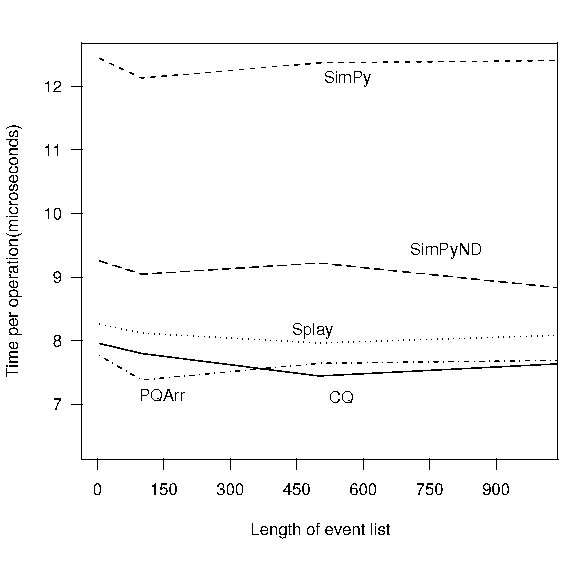
\includegraphics[width=3.0in]{/usr/home/matloff/Research/SimPy/ExpandedGraphs/PhoneLineGraphs1025.jpg}

\end{frame}

\begin{frame}
\frametitle{Call Center Times Per Op, Higher Traffic}

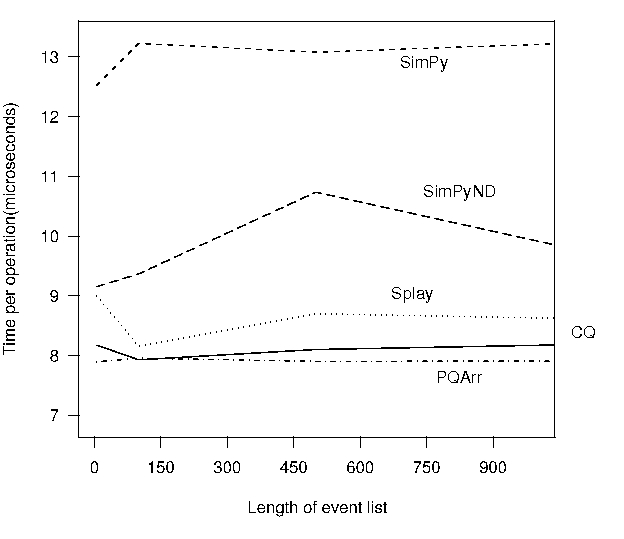
\includegraphics[width=3.0in]{/usr/home/matloff/Research/SimPy/ExpandedGraphs/PhoneLineGraphs2525.jpg}

\end{frame}

\begin{frame}
\frametitle{Hold Model Times Per Op, Smaller COV}

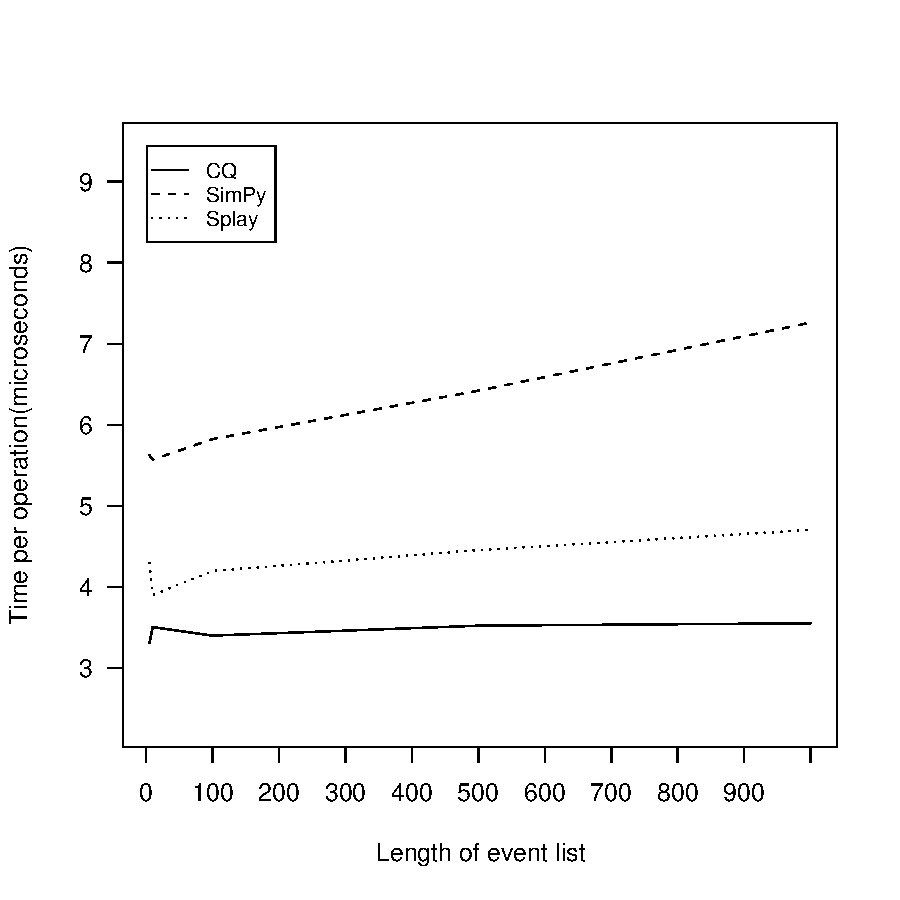
\includegraphics[width=3.0in]{/usr/home/matloff/Research/SimPy/ExpandedGraphs/TestLineGraphs1.pdf} 
\end{frame}

\begin{frame}
\frametitle{Hold Model Times Per Op, Larger COV}

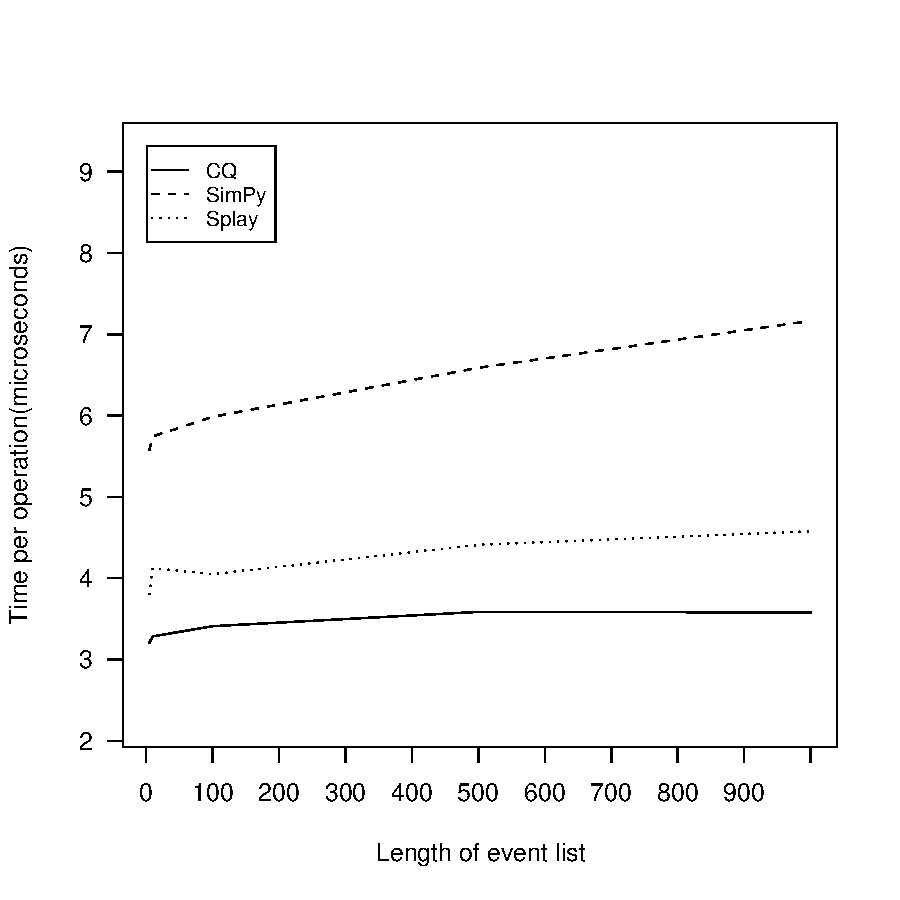
\includegraphics[width=3.0in]{/usr/home/matloff/Research/SimPy/ExpandedGraphs/TestLineGraphs10.pdf} 
\end{frame}

\begin{frame}
\frametitle{Scalability Issues}

\pause

Even though CQ and PQArr were about equal in performance, PQArr appears
not to scale well to larger event sets:

\pause

\vspace{0.3in}

\begin{tabular}{|c|c|c|c|}
\hline
struct & user time & sys. time  & event op. time  \\ \hline
PQArr & 79.47 &  4.50 & 57.87 \\ \pause 
CQ & 33.24 & 3.95 & 12.69 \\ 
\hline
\end{tabular}

\end{frame}

\begin{frame}
\frametitle{Number of Page Faults, Call Center (lower traffic)}

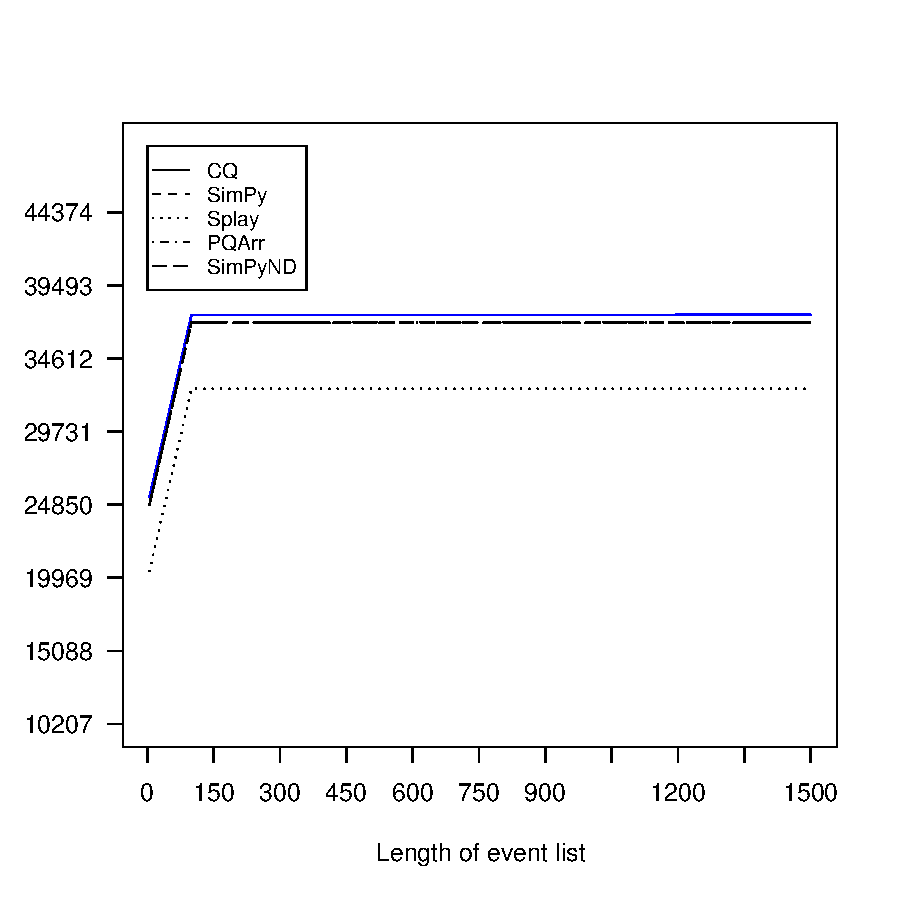
\includegraphics[width=3.0in]{/usr/home/matloff/Research/SimPy/ExpandedGraphs/PhonePageFaultGraphs1025.pdf}

\end{frame}

\begin{frame}
\frametitle{Number of Page Faults, Hold Model (medium COV)}

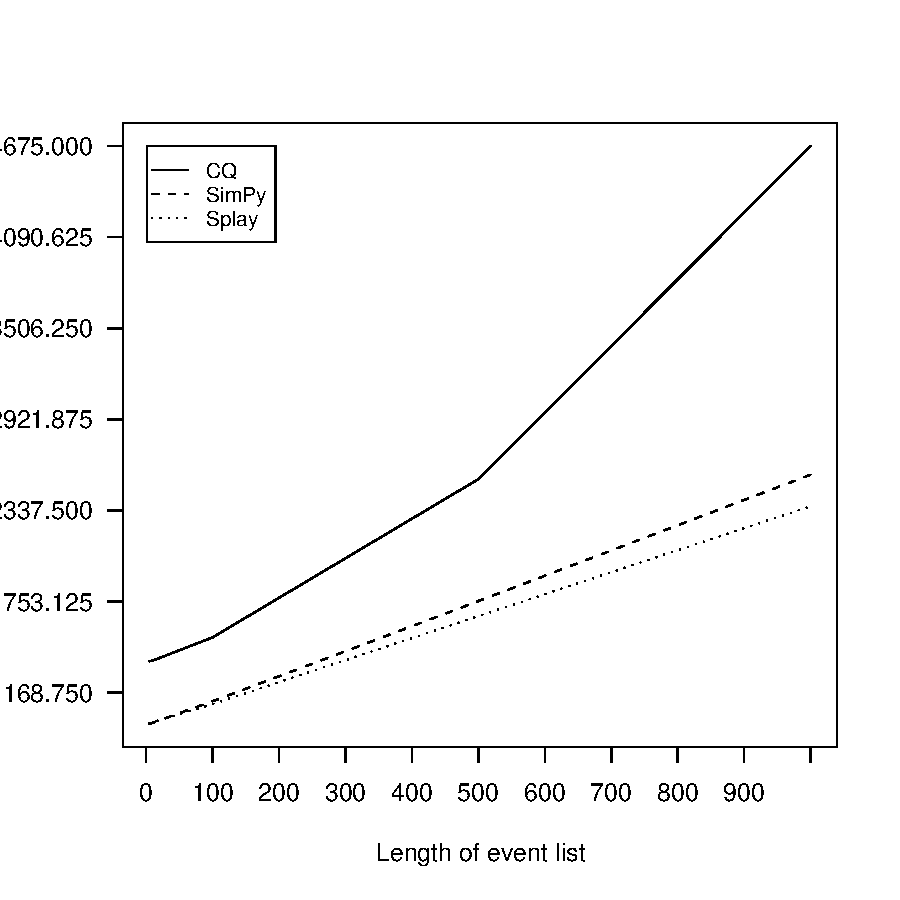
\includegraphics[width=3.0in]{/usr/home/matloff/Research/SimPy/ExpandedGraphs/TestPageFaultGraphs15.pdf}

\end{frame}

\begin{frame}
\frametitle{Discussion of VM Issues}

\begin{itemize}

\pause

\item CQ paging performance poor in our experiments, run on 32-bit PCs
running Linux kernel 2.6.20.

\pause

\item Preliminary experiments on a 64-bit PC, same kernel, suggest
greater variability.

\pause

\item $\therefore$ CQ may do poorly on some systems.

\end{itemize} 

\end{frame}

\begin{frame}
\frametitle{Conclusions and Discussion}

\begin{itemize}

\pause

\item Hybrid interpreted/C approach ``best of both worlds''---transparent
to apps programmer but with better performance

\pause

\item Attention to non-algorithmic issues, e.g. paging, may be
worthwhile.

\pause

\item What about JIT? \pause Tried Pyscho but with disappointing
results.

\end{itemize}

\end{frame}

\end{document}

